
\documentclass[11pt]{article}
\usepackage{IntroAlgorithmsAndLimitations}
\usepackage{graphicx}
\usepackage{float}


\begin{document}

\psHeader{3}{Wed Oct. 1, 2025 (11:59pm)}

Please see the syllabus for the full collaboration and generative AI policy, as well as information on grading, late days, and revisions.

All sources of ideas, including (but not restricted to) any collaborators, AI tools, people outside of the course, websites, ARC tutors, and textbooks other than Hesterberg--Vadhan must be listed on your submitted homework along with a brief description of how they influenced your work. You need not cite core course resources, which are lectures, the Hesterberg--Vadhan textbook, sections, SREs, problem sets and solutions sets from earlier in the semester. If you use any concepts, terminology, or problem-solving approaches not covered in the course material by that point in the semester, you must describe the source of that idea. If you credit an AI tool for a particular idea, then you should also provide a primary source that corroborates it. Github Copilot and similar tools should be turned off when working on programming assignments.

If you did not have any collaborators or external resources, please write 'none.' Please remember to select pages when you submit on Gradescope. A problem set on the border between two letter grades cannot be rounded up if pages are not selected. 

\textbf{Your name: Praneel Khiantani }

\textbf{Collaborators: Mark Li}

\textbf{No. of late days used on previous psets: 0}

\textbf{No. of late days used after including this pset: 1}

\vspace{1em}
The purpose of this problem set is to solidify your understanding of the RAM model (and variants), and the relations between the RAM model, the Word-RAM model, Python programs, and variants. In particular, you will build skills in simulating one computational model by another and in evaluating the runtime of the simulations (both in theory and in practice).


\begin{enumerate}
 
    \item (Simulation in practice: RAMs on Python)
    In the Github repository, we have given you a partially written Python implementation of a universal RAM Model simulator.  Your task is to fill in the missing parts of the code to obtain a complete universal RAM simulator.
     Your simulator should take as input a RAM Program $P$ and an input $x$, and simulate the execution of $P$ on $x$, and return whatever output $P$ produces (if it halts).  The RAM Program $P$ is given as a Python list $[v,C_0,C_1,\ldots,C_{\ell-1}]$, where $v$ is the number of variables used by $P$.  For simplicity, we assume that the variables are named $0,\ldots,v-1$ (rather than having names like ``tmpptr'' and ``insertvalue''), but you can introduce constants to give names to the variables.  The $0$\textsuperscript{th} variable will always be $\inputlen$, the $1$\textsuperscript{st} variable $\outputpointer$, and the $2$\textsuperscript{nd} variable $\outputlen$.  A command $C$ is given in the form of a list of the form $[\cmd]$, $[\cmd,i]$, $[\cmd,i,j]$, or $[\cmd,i,j,k]$, where $\cmd$ is the name of the command and $i,j,k$ are the indices of the variables or line numbers used in the command.  For example,  the command $\var_i = M[\var_j]$ would be represented as $(\READ,i,j)$.  See the Github repository for the precise syntax as well as some RAM programs you can use to test your simulator.


     (done in python file submitted seperately) 

\item (Empirically evaluating simulation runtimes and explaining them theoretically)  

Consider the following two RAM programs:

\begin{algorithm}[H]
\Input{A single natural number $N$ (as an array of length 1)}
\Output{$13^{2^N+1}$ (as an array of length 1)}
\Variables{$\inputlen, \outputpointer, \outputlen, \counter, \result$}
\setcounter{AlgoLine}{-1}
$\zero = 0$\;
$\one = 1$\;
$\thirteen = 13$\;
$\outputlen = 1$\;
$\outputpointer = 0$\;
$\result = 13$\;
$\counter = M[\zero]$\;
\Indp
 IF $\counter == 0$ GOTO \ref{line:done}\; \label{line:loop}
$\result = \result \times \result$\;
$\counter = \counter - \one$\;
IF $\zero == 0$ GOTO \ref{line:loop}\;
\Indm
$\result = \result \times $\thirteen\; \label{line:done}
$M[\outputpointer]=\result$\;
\end{algorithm}

\begin{algorithm}[H]
\Input{A single natural number $N$ (as an array of length 1)}
\Output{$13^{2^N+1} \bmod 2^{32}$ (as an array of length 1)}
\Variables{$\inputlen, \outputpointer, \outputlen, \counter, \result, \temp, \W$}
\setcounter{AlgoLine}{-1}
$\zero = 0$\;
$\one = 1$\;
$\thirteen = 13$\;
$\outputlen = 1$\;
$\outputpointer = 0$\;
$\result = 13$\;
$\W = 2^{32}$\;
$\counter = M[\zero]$\;
\Indp
IF $\counter == 0$ GOTO \ref{line:done2}\; \label{line:loop2}
$\result = \result \times \result$\;
$\temp = \result / \W$\;
$\temp = \temp \times \W$\;
$\result = \result - \temp$\;
$\counter = \counter - \one$\;
IF $\zero == 0$ GOTO \ref{line:loop2}\;
\Indm
$\result = \result \times \thirteen$\;
\label{line:done2}
$\temp = \result / \W$\;
$\temp = \temp \times \W$\;
$\result = \result - \temp$\;
$M[\outputpointer]=\result$\; 
\end{algorithm}


\begin{enumerate}
    \item Exactly calculate (without asymptotic notation) the RAM-model running times of the above algorithms as a function of $N$.
    Which one is faster? \label{itm:RAMtime} 
    
(a) Now, we compute the exact RAM-model step counts for both programs as a function of $N$. For Program A (which is the one without modulo), the setup in lines 0--6 takes 7 steps. The loop test on line 7 is executed $N+1$ times. Inside the loop itself, lines 8--10 are 3 steps long and are repeated $N$ times. After the loop ends, lines 11--12 add 2 more steps. When we add all of this up, we have:
$$T_A(N) = 7 + (N+1) + 3N + 2 = 4N + 10.$$
For Program B (the version with modulo), the setup in lines 0--7 is 8 steps. The loop test on line 8 runs $N+1$ times, and every iteration of the loop body (lines 9--14) is 6 steps, so $6N$ total. Finally, lines 15--19 add 5 more steps. As a whole, we have
$$T_B(N) = 8 + (N+1) + 6N + 5 = 7N + 14.$$
So, in the RAM model, Program A is always faster since $4N+10 < 7N+14$ for all $N \geq 0$.

    
    \item Using your RAM Simulator, run both RAM programs on inputs $N=0,1,2,\ldots,15$ and graph the actual running times (in clock time, not RAM steps).  (We have provided you with some timing and graphing code in the Github repository.) Which one is faster?  \label{itm:realtime}


(b) When we actually run these programs on the Python RAM simulator for $N = 0,1,2,\dots,15$, the runtimes we observe tell us a different story. For $N=0$ both programs are completed instantly, but once $N \geq 1$, Program B consistently runs much faster in wall-clock time when compared to Program A. Program A quickly becomes extremely slow, while in comparison Program B’s runtimes grow smoothly with $N$. Thus in practice, the winner is Program B.

\begin{figure}
    \centering
    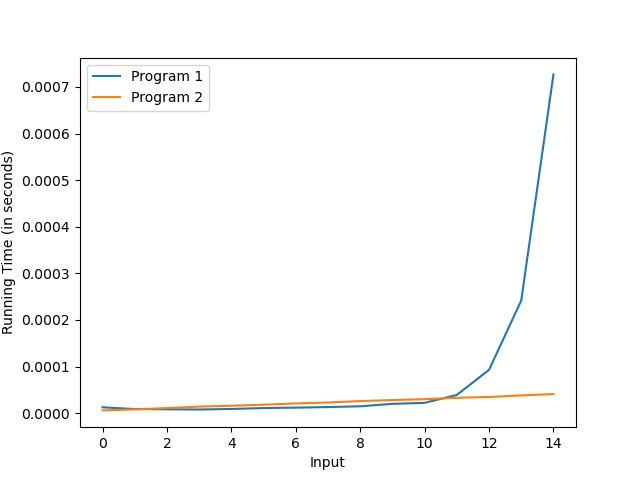
\includegraphics[width=0.5\linewidth]{ps3 graph .png}
    \caption{Graph of Prog 1 v Prog 2 }
    \label{fig:placeholder}
\end{figure}

    
    \item Explain the discrepancies you see between Parts~\ref{itm:RAMtime} and \ref{itm:realtime}.  (Hint: What do we know about the relationship between the RAM and Word-RAM models, and why is it relevant to how efficiently the Python simulation runs?) 

(c) In order to explain this discrepancy, we can remember that the RAM model assumes every arithmetic operation takes unit time, regardless of the size of the operand. That is why Program A looks cheaper in part (a) with less steps per iteration. In practice, Python integers are arbitrary-precision, so the cost of multiplying $B$-bit numbers is superlinear in $B$. Because Program A repeatedly squares its result without reduction, the amount of bits roughly doubles at every iteration, making multiplications more and more costly. Program B, in contrast, reduces modulo $2^{32}$ at every step. This ensures all numbers remain bounded by 32 bits, thus allowing every multiplication to stay cheap. Thus, RAM step counts suggest that A is faster, but the actual performance shows a more Word-RAM–like model, where the size of the operand plays a large factor.

  
 

    \item (optional\footnote{This problem won't make a difference between N, L, R-, and R grades.}) Give a theoretical explanation of the shapes of the runtime curves you see in Part~\ref{itm:realtime}, by providing explicit formulas for the asymptotic runtimes of the two programs (in clock time). You may need to do some research online and/or make guesses about how Python operations are implemented to come up with your estimates. 

        

  
\end{enumerate}





\item (Simulating Word-RAM by RAM)
For every Word-RAM program $P$, there is a RAM program $R$ that simulates $P$ in the following sense.  For every $n \in \N$, input array $x$ of length $n$, word-length $w$, and time bound $t$, $R(x,2^w, \max_i x[i],t)$ should do the following:
\begin{itemize}
    \item If $P[w](x)$ halts without crashing within $t$ steps, then $R$ should halt with the same as the output of $P[w](x)$.
    \item If $P[w](x)$ crashes or fails to halt within its first $t$ steps, then the $R$ should indicate so by halting with $\outputpointer=\outputlen=2^w$.
    \item The runtime of $R$ should be $O(t)$ and the largest memory location accessed by $R$ should be at most $n+t$.
    \item All of the values that $R$'s variables and memory cells hold during the computation should have bitlength at most $O(w+\log \max_i x[i] + \log n)$.
\end{itemize}
Your proof should use an {\em implementation-level} description, similar to the proof that RAM programs can be simulated by ones with at most $c$ registers in Theorem 6.4 from the Hesterberg-Vadhan textbook.  Recall that Word-RAM programs have a finite but changing memory size $S$; you may want to start your simulation by initializing $S$.  Then think about how each operation of a Word-RAM program $P$ can be simulated in a RAM program $R$, taking care of any differences between their semantics in the Word-RAM model vs. the RAM model. Don't forget MALLOC!


Initialization: \\
We start by defining our RAM program $R$ that simulates $P$. 
Word-RAM programs have a finite but changing memory size $S$, and here we can initialize it as $S = n$ as we have an input array of size $n$. 
Since $P$ and $R$ share the same input array $x$, we can set $\inputlen = n$. On initialization, both $\outputpointer = \outputlen = 0$, and they will be updated later by the program before halting. 
Our simulator’s values for $S, \inputlen, \outputlen, \outputpointer$ all match the corresponding values in $P$. 
For memory, we set $M[0] = x_0, M[1] = x_1, \dots M[n - 1] = x_{n-1}$, with all other cells initialized to $0$. 

\vspace{1em}

Maximum Memory: \\
Overall, $S \leq n + t$. We initialized $S = n$, and the only way to increase it is through \texttt{MALLOC}, which extends $S$ by $1$ and sets the new cell to $0$. 
Since at most $t$ steps are executed, we have $S \leq n + t$. 

\vspace{1em}

Execution: \\

Execution begins at $C_0$ with a step counter initialized to $t$. After simulating each Word-RAM instruction, the step counter is decremented. 
If it reaches $0$ before halting, $R$ halts with the special crash output $\outputpointer = \outputlen = 2^w$. 

Each instruction of $P$ is simulated by a constant-size block of RAM instructions:
\begin{itemize}
    \item Arithmetic: $r \gets a \,\text{op}\, b$: perform the operation, then reduce modulo $2^w$.  
    \item Division: if the divisor is $0$, crash ($\outputpointer = \outputlen = 2^w$). Otherwise, perform integer division, then mod $2^w$.  
    \item Read: $r \gets M[a]$: if $a < 0$ or $a \geq S$, crash; otherwise set $r = M[a]$.  
    \item Write: $M[a] \gets b$: if $a < 0$ or $a \geq S$, crash; otherwise $M[a] = b$.  
    \item Malloc: return the current $S$, set $M[S] = 0$, then increment $S$.  
    \item Conditional jumps: update the program counter as in $P$.  
    \item Halt: stop and output the array
    \[
    (M[\outputpointer], M[\outputpointer+1], \dots, M[\outputpointer+\outputlen-1]).
    \]
\end{itemize}

\vspace{1em}

Crash Semantics: \\
Any illegal memory access (under these conditions: $a < 0$ or $a \geq S$), division by $0$, or a timeout is treated as a crash, which halts with
\[
\outputpointer = \outputlen = 2^w.
\]

\vspace{1em}

Runtime: \\
Each Word-RAM instruction is simulated in $O(1)$ steps. Since $R$ simulates at most $t$ steps, the total runtime is $O(t)$. 

\vspace{1em}

Bitlength: \\
\begin{itemize}
    \item Arithmetic values are always reduced modulo $2^w$, so they fit in $w$ bits.  
    \item Input values $x[i]$ may require up to $\log \max_i x[i]$ bits, which are preserved in memory.  
    \item Memory addresses are always $< S \leq n+t$. Since $t \leq 2^w$, this means addresses can be represented with $O(\log n + w)$ bits.  
\end{itemize}
So all variables and memory cells have bitlength bounded by 
\[
O(w + \log \max_i x[i] + \log n).
\]

\vspace{1em}

 \\
Now, we've created a RAM program $R$ that simulates any Word-RAM program $P$ for at most $t$ steps. 
If $P$ halts normally, then $R$ halts with the same output; otherwise $R$ will halt with $\outputpointer = \outputlen = 2^w$. 
The runtime is $O(t)$, the largest memory index used is at most $n+t$, and the bitlength bound holds. 
This implementation matches all of our requirements. 

\end{document}







\item (reflection) Discuss the value (or lack thereof) that you think computational models, and the RAM and Word-RAM models in particular, have for computer science.  All opinions are valid, as long as they show serious thought and are backed by specific justifications.

\item Once you're done with this problem set, please fill out \href{https://forms.gle/PDztMdcoaFxLWV6n8}{this survey} so that we can gather students' thoughts on the problem set, and the class in general. It's not required, but we really appreciate all responses!

\end{enumerate}


\end{document}
